\documentclass[aspectratio=169]{beamer}

\setbeameroption{show notes on second screen}

\usepackage[utf8]{inputenc}
\usetheme{Madrid}
\usecolortheme{beaver}

\usepackage{graphicx}
\graphicspath{ {./Resources/} }

\title{Critical Design Review}       % Title
\author{Austin, Joe, Matt, Kathryn}                     % Team members
\institute{SNHU/CETA}                                   % Institute
\logo{
\includegraphics[height=0.8cm]{../../AJMK_Logo}}  % Our Logo
\titlegraphic{
\includegraphics[height=2.6cm]{Stencil.png}} % Title graphic

\begin{document}

\frame{\titlepage} % Draw the title page
\note{Title page notes here.}

\section{Introduction}

\begin{frame}
    \frametitle{Agenda}

    \begin{columns}
    \begin{column}{0.48\textwidth}
        \setcounter{tocdepth}{1} % Prof requested we do this
        {\tableofcontents}
    \end{column}

    \begin{column}{0.48\textwidth}
        \begin{center}
            
\includegraphics[height=3cm]{../../AJMK_Logo}
            
\includegraphics[height=3cm]{Stencil.png}
        \end{center}
    \end{column}
    \end{columns}

\note{
\huge Everyone \normalsize

\begin{itemize}
 \item We'll do questions at the end
 \item Page numbers are in the bottom right, remember to note what page you'd like us to go back to!
\end{itemize}
}
\end{frame}

\section{ConOps Summary}
\begin{frame}
    \frametitle{ConOps Summary}

    \begin{columns}

    \begin{column}{0.34\textwidth}
        Stakeholders
        \begin{itemize}
         \item SNHU
         \item Professors
         \item Industrial Trainers
         \item Parts and manufacturers
        \end{itemize}

        Users
        \begin{itemize}
         \item Pendulum Team
         \item Educators
        \end{itemize}
    \end{column}

    \begin{column}{0.65\textwidth}
        \begin{block}{Operating Modes}
            \begin{enumerate}
            \item Off mode
            \item Idle mode
            \item Spinup mode
            \item Demo mode
            \item User PID mode
            \end{enumerate}
        \end{block}

        \begin{block}{System Description}
            \small{An inverted pendulum is a type of PID Demonstrator, where a simple PID loop
            controls and minimizes the error in a system, in this case, the error is the angle of the pendulum. A perfectly tuned PID loop will hover the pendulum.}
            \textbf{Perfectly Still}.
        \end{block}
    \end{column}
\end{columns}

\note{
\huge Matt \normalsize

\begin{itemize}
 \item So our stakeholders include SNHU, our professors, industrial trainers and of course the people who supply parts and manfucacture our product.
 \item At the moment, we're the ones manufacturing it but in the future it could be different.
 \item Our users are us and educators who might want to use this product to teach the fundamnetals of PID
 \item It has a few modes, Off, Idle, Spinup, Demo and user PID mode. The last two are where the pendulum self-balances
 \item Its almost like a game, the system is naturally unstable, the pendulum wants to fall, but a properly tuned PID loop can keep it upright!
\end{itemize}
}

\end{frame}

\begin{frame}
    \frametitle{ConOps (cont.)}

    \begin{columns}
        \begin{column}{0.48\textwidth}
            \begin{block}{Operation and Support Environment}
                \begin{itemize}
                 \item Built from COTS (common off the shelf) parts
                 \item Designed to be serviced
                 \item Constant Uptime
                 \item Low power modes
                \end{itemize}
            \end{block}
        \end{column}

        \begin{column}{0.48\textwidth}
            \begin{block}{Impact considerations}
                \begin{itemize}
                 \item Requiring physical space, either for storage or use.
                 \item Being a hazard and risking misuse.
                 \item Generating pollutants and disposal.
                \end{itemize}
            \end{block}
        \end{column}
    \end{columns}

\note{
\huge Matt \normalsize

\begin{itemize}
 \item Being built from COTS parts allows us to easily replace components and design service schedules
 \item We also have plans for a low power mode and folding or removable legs to decrease electrical and physical footprint.
\end{itemize}
}

\end{frame}

\begin{frame}
    \frametitle{Summary of Trade Studies}

    Content here

    \note{
        Notes here
    }
\end{frame}


\begin{frame}
    \frametitle{Functional Requirements}

    Content here

    \note{
        Notes here
    }
\end{frame}

\begin{frame}
    \frametitle{Performance Requirements}

    Content here

    \note{
        Notes here
    }
\end{frame}


\begin{frame}
    \frametitle{Other Requirements}

    Content here

    \note{
        Notes here
    }
\end{frame}


\begin{frame}
    \frametitle{System Design}

    Content here

    \note{
        Notes here
    }
\end{frame}


\begin{frame}
    \frametitle{Functional Block Diagram}

    Content here

    \note{
        Notes here
    }
\end{frame}


\begin{frame}
    \frametitle{Bill Of Materials}

    Content here

    \note{
        Notes here
    }
\end{frame}


\begin{frame}
    \frametitle{Safety}

    Content here

    \note{
        Notes here
    }
\end{frame}


\begin{frame}
    \frametitle{Impact Considerations}

    Content here

    \note{
        Notes here
    }
\end{frame}


\begin{frame}
    \frametitle{Calibration and Maintenance}

    Content here

    \note{
        Notes here
    }
\end{frame}


\begin{frame}
    \frametitle{Verification Plan}

    Content here

    \note{
        Notes here
    }
\end{frame}


\begin{frame}
    \frametitle{Phase D}

    Content here

    \note{
        Notes here
    }
\end{frame}


\begin{frame}
    \frametitle{Ethics}

    Content here

    \note{
        Notes here
    }
\end{frame}


\section{Diagrams}
\subsection{Block Diagrams}
\begin{frame}
    \frametitle{Block Diagram}

    \begin{columns}
        \begin{column}{0.70\textwidth}
            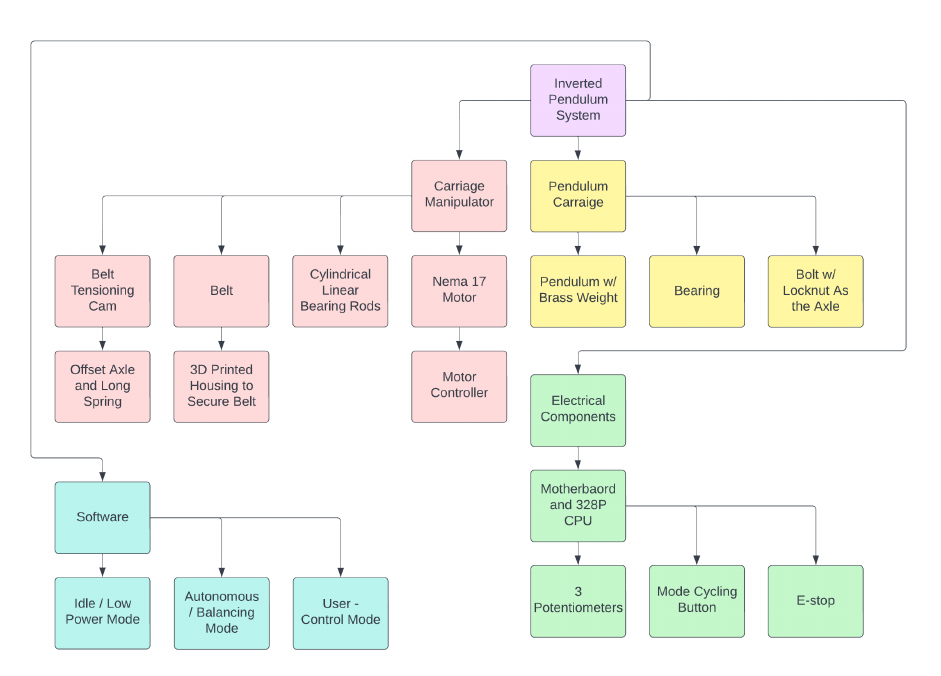
\includegraphics[height=7cm]{BlockDiagram}
        \end{column}

        \begin{column}{0.30\textwidth}
            \begin{block}{Block Diagram}
                The block diagram details the electrical, mechanical and software components.
                And their relationship to each other.
            \end{block}
        \end{column}
    \end{columns}

\note{
\huge Matt \normalsize

\begin{itemize}
 \item Our block diagram shows how our software, hardware and electronics may interact in a final system
\end{itemize}
}

\end{frame}

\subsection{Operations}
\begin{frame}
    \frametitle{Operations}

    \begin{columns}
        \begin{column}{0.30\textwidth}
            \begin{block}{Operations}
                The Operations diagram details the physical and general controls.
            \end{block}
        \end{column}

        \begin{column}{0.70\textwidth}
            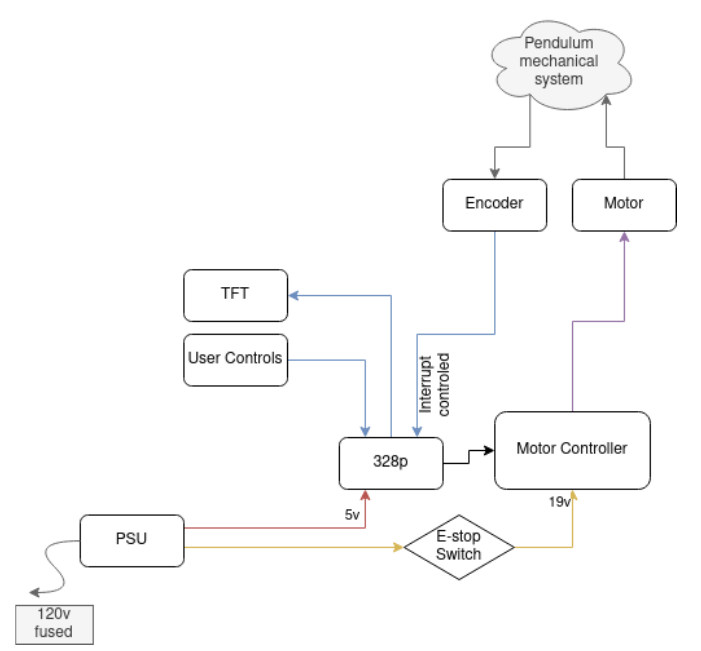
\includegraphics[height=7cm]{Operations}
        \end{column}
    \end{columns}

\note{
\huge Joe \normalsize

\begin{itemize}
 \item The operations chart details our physical and general controls like the tft screen
 \item the buttons
 \item the motor controller and encoders
\end{itemize}
}

\end{frame}

\subsection{Software}
\begin{frame}
    \frametitle{Software Flowchart}

    \begin{columns}
        \begin{column}{0.72\textwidth}
            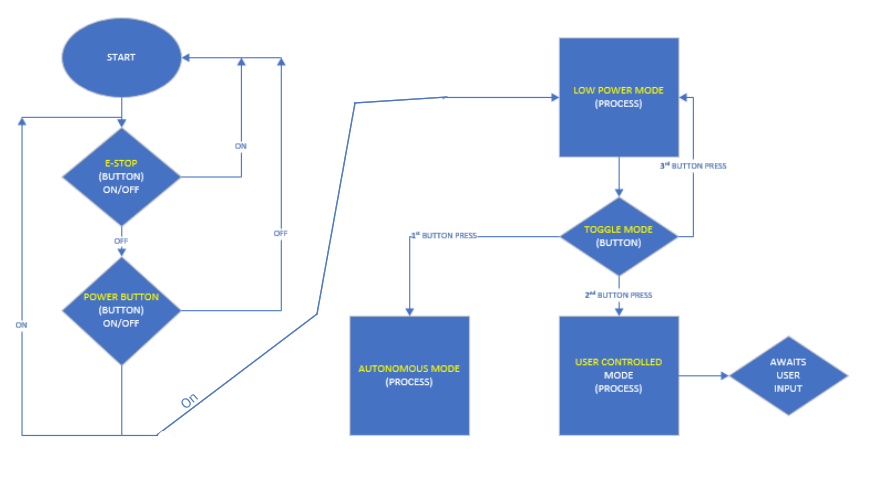
\includegraphics[width=11cm]{SoftwareFlowchart}
        \end{column}

        \begin{column}{0.28\textwidth}
            \begin{block}{Software Flowchart}
                The software flowchart is an overview of all the software functions of our
                proposed product.
            \end{block}
        \end{column}
    \end{columns}

\note{
\huge Austin \normalsize

\begin{itemize}
 \item Our software flowchart details how the PID control scheme will be interactable by the users
\end{itemize}
}

\end{frame}


\section{End}
\begin{frame}
    \frametitle{End}

    \begin{block}{}
        \begin{center}
            \Huge Questions and Comments?
        \end{center}
    \end{block}

    \begin{center}
        Find the source code for this document, and the rest of our designs, firmware, hardware
        and notes on GitHub!

        
\includegraphics[height=2cm]{github_qr}
    \end{center}

\note{
\begin{itemize}
 \item So please if you have any questions we would love to hear them.
 \item All of our software, CAD, hardware and design docs are licensed under
 \item \huge The MIT Open Source License \normalsize and available via git.
 \item If you have a specific slide in mind we can go back to it!
\end{itemize}
}
\end{frame}

\begin{frame}
    \frametitle{Close Ups}

    Put some close up shots here
\end{frame}


\end{document}
